\documentclass[11pt]{article}
\usepackage[a4paper,margin=0.9in]{geometry}
\usepackage{amsmath,amssymb}
\usepackage{xcolor}
\usepackage{booktabs}
\usepackage{tikz}
\usepackage{parskip}
\usepackage{titlesec}
\usetikzlibrary{positioning, arrows.meta, calc, fit}

\titleformat{\section}{\large\bfseries}{\thesection}{0.6em}{}

\title{Hulse Model A --- where is the 3-D input $u$ injected?}
\author{Internal note, connectome-gnn project}
\date{2026-05-13}

\begin{document}
\maketitle

\section*{Architecture at a glance}

\begin{center}
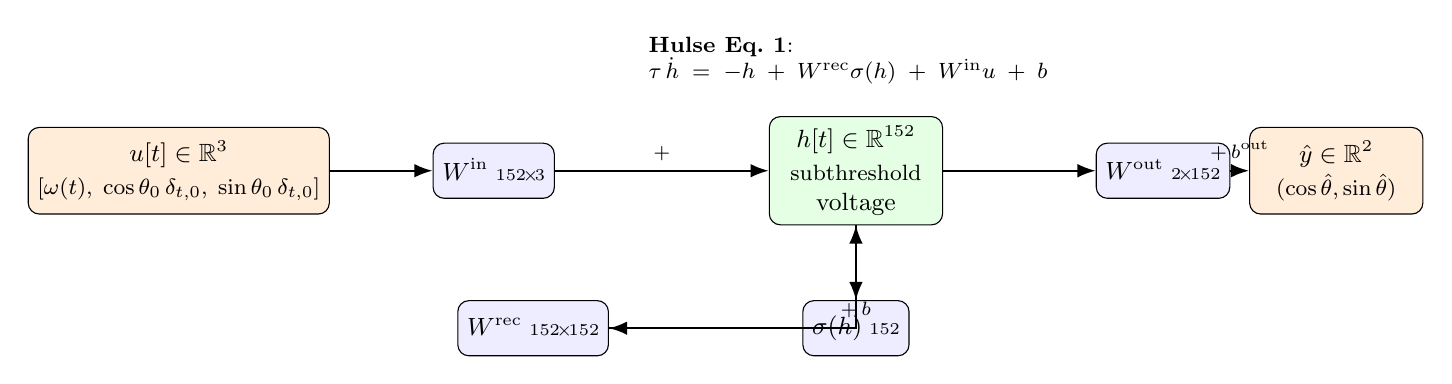
\begin{tikzpicture}[
  every node/.style={font=\small},
  block/.style={draw, rounded corners, minimum width=2.2cm, minimum height=1.1cm, align=center},
  mat/.style={draw, fill=blue!7, rounded corners, minimum width=1.3cm, minimum height=0.7cm, font=\small\ttfamily},
  arrow/.style={-Latex, thick}
]

% Input nodes
\node[block, fill=orange!15] (u) at (0, 0)
   {$u[t]\in\mathbb{R}^{3}$\\[1pt]
    \footnotesize $[\omega(t),\;\cos\theta_0\,\delta_{t,0},\;\sin\theta_0\,\delta_{t,0}]$};

% Win projection
\node[mat] (Win) at (4.0, 0) {$W^{\mathrm{in}}\;{\scriptstyle 152\!\times\!3}$};
\draw[arrow] (u) -- (Win);

% Hidden state and recurrent loop
\node[block, fill=green!10] (h) at (8.6, 0)
   {$h[t]\in\mathbb{R}^{152}$\\[1pt]
    \footnotesize subthreshold\\voltage};
\draw[arrow] (Win) -- (h) node[midway, above, font=\scriptsize] {$+$};

% Sigmoid then W_rec loop
\node[mat] (sig) at (8.6, -2.0) {$\sigma(h)\;{\scriptstyle 152}$};
\node[mat] (Wrec) at (4.5, -2.0) {$W^{\mathrm{rec}}\;{\scriptstyle 152\!\times\!152}$};
\draw[arrow] (h) -- (sig);
\draw[arrow] (sig) -- (Wrec);
\draw[arrow] (Wrec) -| (h) node[midway, above, font=\scriptsize] {$+\,b$};

% Readout
\node[mat] (Wout) at (12.5, 0) {$W^{\mathrm{out}}\;{\scriptstyle 2\!\times\!152}$};
\node[block, fill=orange!15] (y) at (14.7, 0)
   {$\hat y\in\mathbb{R}^{2}$\\[1pt]
    \footnotesize $(\cos\hat\theta,\sin\hat\theta)$};
\draw[arrow] (h) -- (Wout);
\draw[arrow] (Wout) -- (y) node[midway, above, font=\scriptsize] {$+\,b^{\mathrm{out}}$};

% Annotation: ODE
\node[align=left, font=\footnotesize] at (8.5, 1.4)
   {\textbf{Hulse Eq.~1}: \\
    $\tau\,\dot h \;=\;-h \;+\; W^{\mathrm{rec}}\sigma(h)
    \;+\; W^{\mathrm{in}} u \;+\; b$};

\end{tikzpicture}
\end{center}

\section*{Where the injection happens (in code)}

\begin{center}\small\ttfamily
hulse\_cx\_teacher.py, \texttt{HulseCxRNN.forward}, lines 168--181:
\end{center}
\vspace{-0.3em}
{\small
\begin{verbatim}
for t in range(T):
    r   = torch.sigmoid(h)                    # (B, 152)
    rec = r @ self.W_rec.t()                  # (B, 152)
    inp = u[:, t, :] @ self.W_in.t()          # (B, 152)  <-- injection point
    dh  = -h + rec + inp + self.b
    h   = h + (dt / tau) * dh
\end{verbatim}
}

\section*{Yes, 152$\times$152 is the recurrent network}

The recurrent matrix $W^{\mathrm{rec}}\in\mathbb{R}^{152\times 152}$ is the
``connectome'' --- 152 neurons drawn from the Beiran hemibrain CX loader
(EPG, EPGt, PEN\_a, PEN\_b, $\Delta_7$, PEG types). Each row is one
postsynaptic unit, each column is one presynaptic unit. The Dale-style
sign mask is already baked into the connectome template
$W^{\mathrm{con}}$ used as the regulariser target.

\section*{Full parameter inventory}

\begin{center}\small
\begin{tabular}{lll}
\toprule
\textbf{Tensor} & \textbf{Shape} & \textbf{Role} \\
\midrule
$h$ (state)       & $(B,\,152)$        & subthreshold voltage \\
$W^{\mathrm{rec}}$ & $(152,\,152)$     & recurrent weights (the connectome) \\
$W^{\mathrm{in}}$  & $(152,\,3)$       & input projection from the 3-channel $u$ \\
$b$               & $(152,)$           & recurrent biases (initial value 1) \\
$W^{\mathrm{out}}$ & $(2,\,152)$       & readout to $(\cos\theta,\sin\theta)$ \\
$b^{\mathrm{out}}$ & $(2,)$             & readout bias \\
$u$ (input)       & $(B,\,T,\,3)$      & OU velocity + initial-heading impulse \\
$\hat y$ (output) & $(B,\,T,\,2)$      & predicted head direction \\
\bottomrule
\end{tabular}
\end{center}

For one $T=100$-step trial in the default batch ($B=100$), the network
sees $300$ scalar inputs (3 channels $\times$ 100 timesteps) and
produces $200$ scalar outputs (2 readouts $\times$ 100 timesteps),
mediated by $152^{2}=23{,}104$ recurrent weights plus
$152\times 3=456$ input weights and $2\times 152=304$ readout weights.

\end{document}
